\documentclass[a4paper,12pt]{article}
\usepackage[french]{babel} 
\usepackage[T1]{fontenc}
%\usepackage[ansinew]{inputenc}
\usepackage[utf8]{inputenc}
\usepackage[top=3cm, bottom=3cm, left=2.3cm,right=2cm]{geometry}
\usepackage{graphicx}
\usepackage{color}
\usepackage{listings}
%\usepackage{marvosym}
%\usepackage{yfonts}
\usepackage[normalem]{ulem}
\usepackage{verbatim}
\usepackage{listings}
\usepackage{float}
%\renewcommand{\thesection}{\arabic{section}}
\usepackage{array} % pour les tableaux
\usepackage{amsmath} % pour les équations
\usepackage{float}
\usepackage{hyperref}	% crée des liens dans le pdf
\hypersetup{					% colorise les liens du pdf
  colorlinks=true,
  urlcolor=black
	citecolor=black,
  linkcolor=black,
  urlcolor=blue
}
\usepackage{url}			% change la police des url (utilisation : \url{http://asdf.ch})
\definecolor{dkgreen}{rgb}{0,0.6,0}
\definecolor{gray}{rgb}{0.5,0.5,0.5}
\definecolor{mauve}{rgb}{0.58,0.01,0.82}
%[babel=true]
\usepackage{csquotes}
\lstset{ %
  language=C,                % the language of the code
  basicstyle=\footnotesize,           % the size of the fonts that are used for the code
  numbers=left,                   % where to put the line-numbers
  numberstyle=\tiny\color{gray},  % the style that is used for the line-numbers
  stepnumber=1,                   % the step between two line-numbers. If it's 1, each line 
                                  % will be numbered
  numbersep=5pt,                  % how far the line-numbers are from the code
  backgroundcolor=\color{white},      % choose the background color. You must add \usepackage{color}
  showspaces=false,               % show spaces adding particular underscores
  showstringspaces=false,         % underline spaces within strings
  showtabs=false,                 % show tabs within strings adding particular underscores
  frame=single,                   % adds a frame around the code
  rulecolor=\color{black},        % if not set, the frame-color may be changed on line-breaks within not-black text (e.g. commens (green here))
  tabsize=2,                      % sets default tabsize to 2 spaces
  captionpos=b,                   % sets the caption-position to bottom
  breaklines=true,                % sets automatic line breaking
  breakatwhitespace=false,        % sets if automatic breaks should only happen at whitespace
  title=\lstname,                   % show the filename of files included with \lstinputlisting;
                                  % also try caption instead of title
  keywordstyle=\color{blue},          % keyword style
  commentstyle=\color{dkgreen},       % comment style
  stringstyle=\color{mauve},         % string literal style
  escapeinside={\%*}{*)},            % if you want to add a comment within your code
  morekeywords={*,...}               % if you want to add more keywords to the set
}

%Table of content with dot
\usepackage{etoolbox}
\makeatletter
\patchcmd{\l@section}
{\hfil}
{\leaders\hbox{\normalfont$\m@th\mkern \@dotsep mu\hbox{.}\mkern \@dotsep mu$}\hfill}
{}{}
\makeatother

%no indentation
\setlength{\parindent}{0cm}

%en-tête
\usepackage{fancyhdr}
\lhead{SEEE}
\chead{}
\rhead{\today}
\pagestyle{fancy}

% Title Page
\title{\Huge{\textsc{Systèmes d'exploitation et environnements d'exécution embarqués}} \\ 
	\Huge{\textbf{Rapport de laboratoire}} \\
	\huge{Master HES-SO}}
\author{Émilie \textsc{Gsponer}, Grégory \textsc{Emery} }
\date{\today \\
	version 1.0}

%-------------------------début du document-------------------------------------
\begin{document}

\maketitle % page de garde
\newpage
\tableofcontents % table des matières
\newpage
\section{Introduction REPTAR}
\subsection{Mise en place de l'environnement, utilisation de git}
\textbf{a) Donnée: }Il faut tout d'abord récupérer le dépôt étudiant pour les laboratoires SEEE à l'aide de la commande
suivante (via une fenêtre de terminal):
\begin{lstlisting}
$ git clone firstname.lastname@eigit.heig-vd.ch:/home2/reds/seee/seee_student
\end{lstlisting}
\textbf{Travail réalisé: }
Nous n'avions pas les droits d'accès pour le dépôt git, nous l'avons donc téléchargé, puis extrait depuis le lien:
\url{https://drive.switch.ch/index.php/s/TbHxQZtmO9IVdkb}.\\
Le dossier seee\_student a ensuite été placé dans: /home/redsuser/\\

\textbf{b) Donnée: }Lancez Eclipse et ouvrez le workspace seee\_student. Vous devriez obtenir la liste des projets (à
gauche). Chaque projet a un lien symbolique dans la racine du workspace. \\\\
\textbf{Travail réalisé: }
En introduisant le path du dossier seee\_student comme workspace au lancement d'Eclipse, nous obtenons la liste de projets suivante:
\begin{figure}[H]
	\begin{center}
		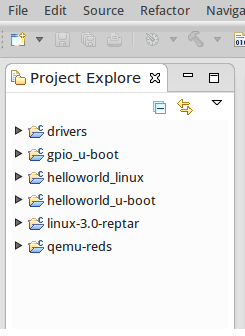
\includegraphics[height=7cm]{img/eclipseProjet.png}
		\caption{Liste des projets}
		\label{eclipseProjet}
	\end{center}
\end{figure}
\textbf{c) Donnée: }Compilez maintenant l'émulateur Qemu. Dans une fenêtre de terminal, lancez la commande
suivante à partir de votre répertoire seee\_student : 
\begin{lstlisting}
$ make qemu
\end{lstlisting}
\textbf{Travail réalisé: }
Vu que nous n'avons pas téléchargé le dossier de projets depuis git, il faut nettoyer le contenu du dossier avec clean ou distclean avant de pourvoir utiliser qemu. Le make qemu prend quelques instants.\\
\begin{lstlisting}
redsuser@vm-reds-2015s2:~/seee_student$ make clean
redsuser@vm-reds-2015s2:~/seee_student$ make qemu
...
make[1]: Leaving directory `/home/redsuser/seee_student/qemu-reds'
redsuser@vm-reds-2015s2:~/seee_student$
\end{lstlisting}
\subsection{Démarrage de Qemu}
\textbf{a) Donnée: }Depuis Eclipse, lancez le debugger avec la configuration de debug « qemu-reds Debug ». Dans la
fenêtre Console, vous pourrez entrer directement des commandes de U-boot (tapez help par
exemple). \\\\
\textbf{Travail réalisé: }
\begin{figure}[H]
	\begin{center}
		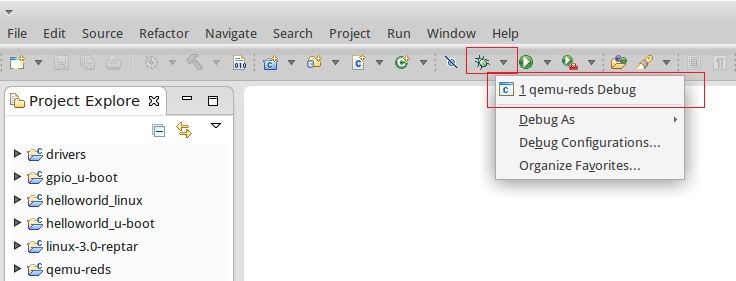
\includegraphics[height=7cm]{img/manip2Intro.png}
		\caption{Lancement d'Eclipse en mode Debug}
		\label{eclipseDebug}
	\end{center}
\end{figure}
\textbf{Remarque: }Après le lancement du Debug, il faut changer d'onglet en haut à droite en choisissant \textit{Debug} pour avoir la console. Ce changement d'onglet ne se fait pas automatiquement.
\begin{figure}[H]
	\begin{center}
		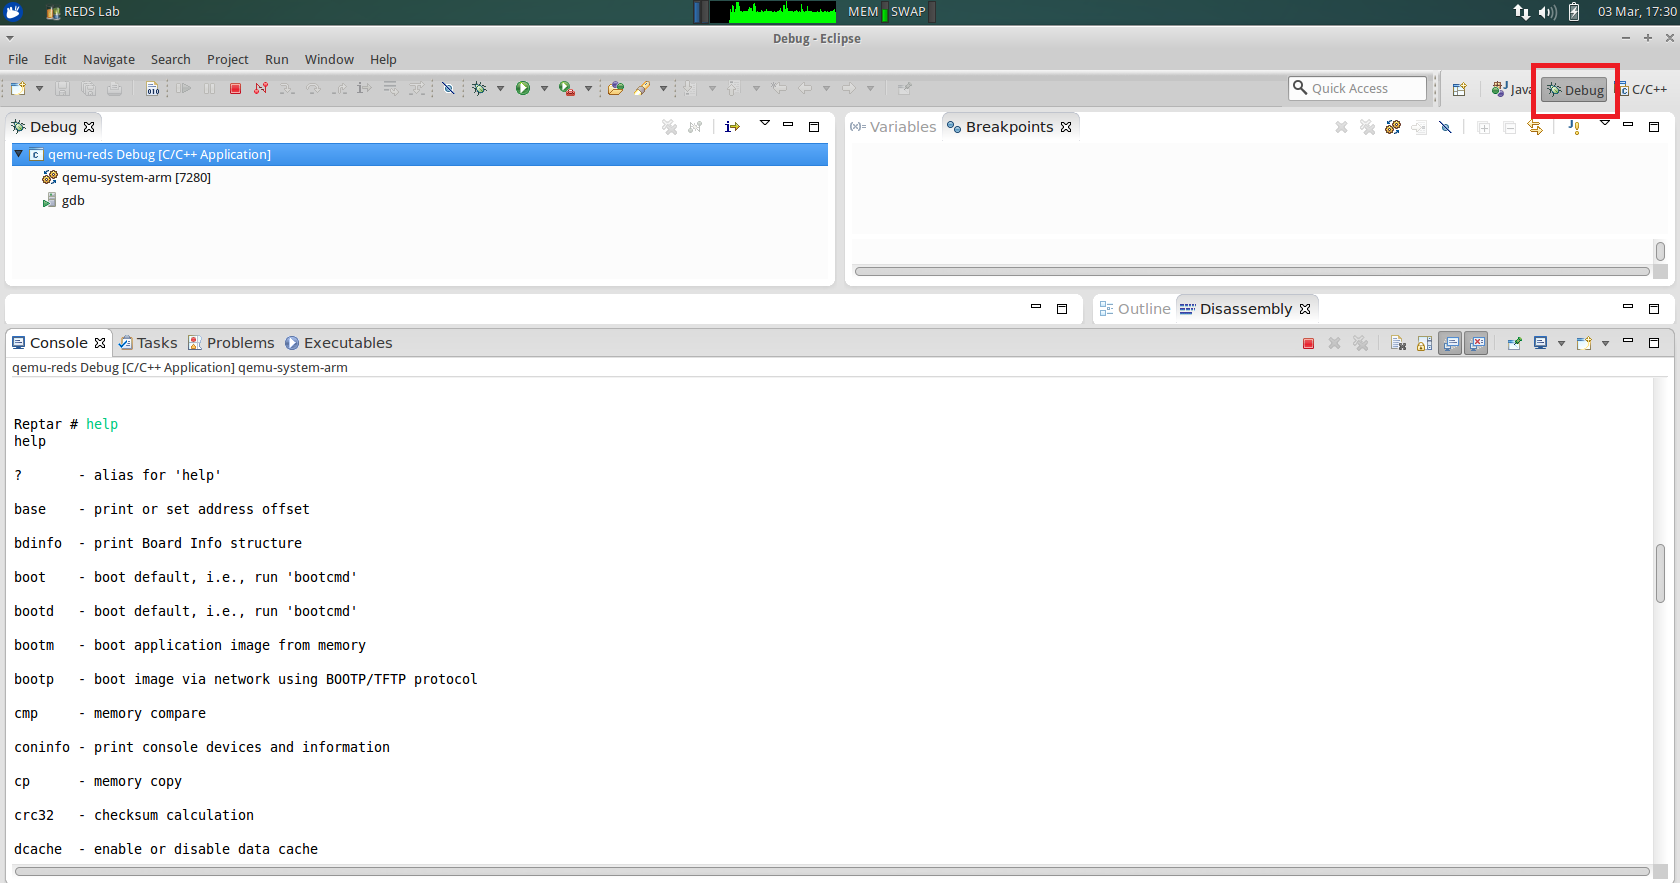
\includegraphics[width=18cm]{img/ubootCommand.png}
		\caption{Command help dans l'U-boot}
		\label{ubootCommand}
	\end{center}
\end{figure}
\textbf{b) Donnée: } Interrompez l'exécution du programme en cliquant sur l'icône pause. Identifiez la ligne en cours d'exécution dans le code source. \\\\
\textbf{Travail réalisé: }En interrompant le programme avec le bouton \textit{suspend}, on obtient la vue assembleur ci-dessous. L'environnement essaie d'ouvrir le fichier ppoll.c, on est donc en attente d'un événement. Le programme est interrompu après un syscall.
\begin{figure}[H]
	\begin{center}
		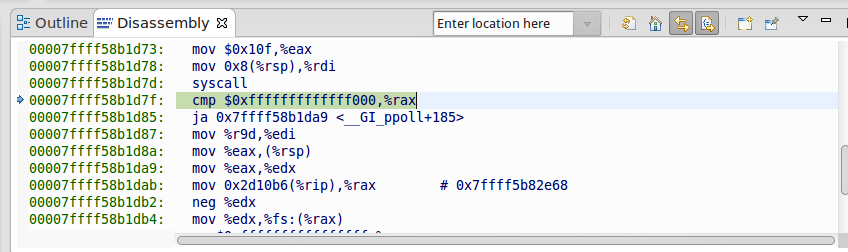
\includegraphics[width=18cm]{img/ubootAsm.png}
		\caption{Command help dans l'U-boot}
		\label{ubootAsm}
	\end{center}
\end{figure}
\textbf{c) Donnée: } Stoppez l'exécution, et dans une fenêtre de commande, démarrez qemu à l'aide du script stf (en
tapant ./stf) dans le répertoire racine. Vous arrivez dans U-boot. \\\\
\textbf{Travail réalisé: }Cette partie n'a plus rien avoir avec Eclipse, on peut le fermer et lancer un terminal.
Avec la commande \textit{stf} tapée à la racine du répertoire seee\_student, on arrive au même point qu'en lançant le Debug dans Eclipse. On peut également essayer la commande \textit{help}
\begin{lstlisting}
redsuser@vm-reds-2015s2:~/seee_student$ ./stf
WARNING: Image format was not specified for 'filesystem/flash' and probing guessed raw.
...

Reptar # help
?       - alias for 'help'
base    - print or set address offset
bdinfo  - print Board Info structure
boot    - boot default, i.e., run 'bootcmd'
bootd   - boot default, i.e., run 'bootcmd'
bootm   - boot application image from memory
bootp   - boot image via network usi
...
\end{lstlisting}
\subsection{Tests avec U-boot}
\textbf{a) Donnée: }Dans U-boot, listez les variables d'environnement avec la commande printenv. Observez les
variables prédéfinies « tftp1, tftp2 et goapp ». Ces variables définissent des commandes U-boot qui
peuvent être exécutées à l'aide de la commande run (par exemple run tftp1).
La commande go <addr> permet de lancer l'exécution à l'adresse physique <addr>.
Vous pouvez définir/modifier vos propres variables et les sauvegarder dans la flash émulée avec la
commande saveenv (seulement avec le lancement via stf). \\\\
\textbf{Travail Réalisé: }Après être entré dans l'U-boot avec \textit{stf}, nous avons pu lister les variables d'environnement suivantes:
\begin{lstlisting}
redsuser@vm-reds-2015s2:~$ cd seee_student/
redsuser@vm-reds-2015s2:~/seee_student$ ./stf
WARNING: Image format was not specified for 'filesystem/flash' and probing guessed raw.
...
goapp=go 0x81600000
...
tftp1=tftp helloworld_u-boot/helloworld.bin
tftp2=tftp gpio_u-boot/gpio_u-boot.bin

Environment size: 930/4092 bytes
Reptar # 
\end{lstlisting}
Les variables \textit{tftp1} et \textit{tftp2} sont des alias permettant de lancer des applications, la variable goapp est un alias permettant de lancer l'exécution de l'adresse physique 0x81600000. Elle définit l'adresse de début des applications. Voici un exemple d'utilisation de ces variables:
\begin{lstlisting}
redsuser@vm-reds-2015s2:~$ cd seee_student/
redsuser@vm-reds-2015s2:~/seee_student$ cd helloworld_u-boot/
redsuser@vm-reds-2015s2:~/seee_student/helloworld_u-boot$ make
...
redsuser@vm-reds-2015s2:~/seee_student/helloworld_u-boot$ cd ../gpio_u-boot/
redsuser@vm-reds-2015s2:~/seee_student/gpio_u-boot$ make
...
redsuser@vm-reds-2015s2:~/seee_student/gpio_u-boot$ cd ..
redsuser@vm-reds-2015s2:~/seee_student$ ./stf 
WARNING: Image format was not specified for 'filesystem/flash' and probing guessed raw.
...
Reptar # run tftp1
smc911x: detected LAN9118 controller
smc911x: phy initialized
smc911x: MAC e4:af:a1:40:01:fe
Using smc911x-0 device
TFTP from server 10.0.2.2; our IP address is 10.0.2.10
Filename 'helloworld_u-boot/helloworld.bin'.
Load address: 0x81600000
Loading: #
done
Bytes transferred = 776 (308 hex)

Reptar # run goapp
## Starting application at 0x81600000 ...
Example expects ABI version 6
Actual U-Boot ABI version 6
Hello World
argc = 1
argv[0] = "0x81600000"
argv[1] = "<NULL>"
Hit any key to exit ... 
## Application terminated, rc = 0x0

Reptar # run tftp2
smc911x: detected LAN9118 controller
smc911x: phy initialized
smc911x: MAC e4:af:a1:40:01:fe
Using smc911x-0 device
TFTP from server 10.0.2.2; our IP address is 10.0.2.10
Filename 'gpio_u-boot/gpio_u-boot.bin'.
Load address: 0x81600000
Loading: #
done
Bytes transferred = 3080 (c08 hex)

Reptar # run goapp
## Starting application at 0x81600000 ...
Start of the GPIO U-boot Standalone Application
Stop of the GPIO U-boot Standalone Application
## Application terminated, rc = 0x0
Reptar #
\end{lstlisting}
La commande run tftp<x> charge une application à l'adresse 0x81600000, tandis que run goapp va exécuter l'application à cette adresse comme le montre l'exemple ci-dessus.\\\\
\textbf{b) Donnée: }La production de l'exécutable helloworld\_u-boot s'effectue en tapant la commande make dans le
répertoire contenant les sources du programme. Ensuite, vous pouvez transférer le fichier (extension
.bin) dans U-boot et exécuter le binaire (aidez-vous des variables d'environnement prédéfinies). \\\\
\textbf{Travail réalisé: } Ce point a été fait en même temps que le précédent.\\

\textbf{c) Donnée: } Testez le debugger dans Eclipse avec le projet helloworld\_u-boot. Mettez un breakpoint dans le
code source au démarrage du programme, et lancez le debugger avec la configuration de debug
« helloworld\_u-boot Debug ». \\\\
\textbf{Travail Réalisé: } Il faut que U-boot soit démarré dans un terminal externe avec \textit{stf} pour que la manipulation fonctionne avec Eclipse.
\begin{figure}[H]
	\begin{center}
		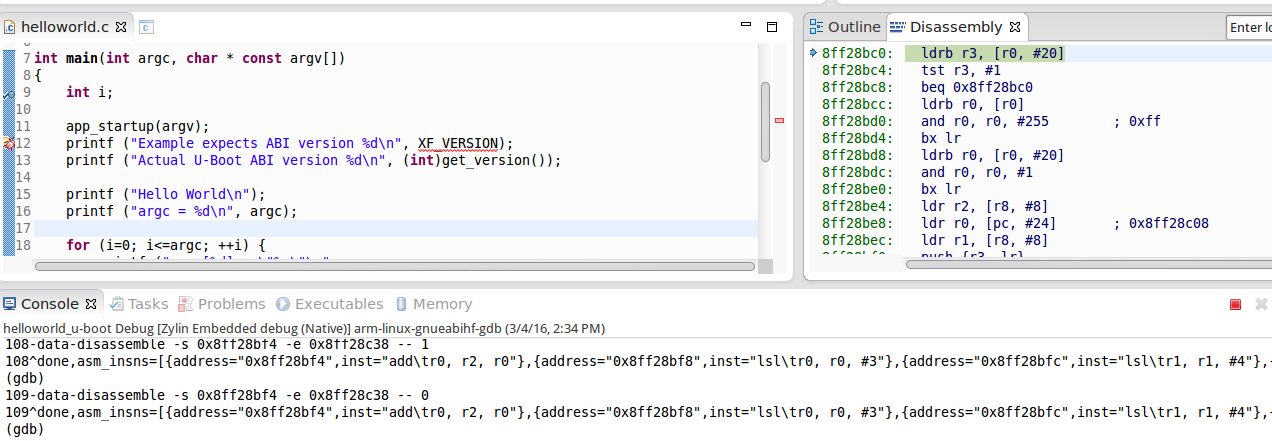
\includegraphics[width=18cm]{img/ubootCommand2.png}
		\caption{Debug d'hello\_world\_u-boot}
		\label{ubootComm2}
	\end{center}
\end{figure}
\textbf{Remarque: }\color{red}Qemu se comporte comme un serveur GDB, ce qui permet à Eclipse  de communiquer avec lui et de debugger des applications...à retravailler\color{black}
\subsection{Tests avec Linux}
\textbf{a) Donnée: }Lancez le script ./deploy qui permettra de déployer le noyau Linux dans la sdcard virtuelle (ignorez
l'erreur due à l'absence de certains fichiers). \\\\
\textbf{Travail réalisé: }
\begin{lstlisting}
redsuser@vm-reds-2015s2:~/seee_student$ ./deploy 
Deploying into reptar rootfs ...
Mounting filesystem/sd-card.img...
[sudo] password for redsuser: 
SD card partitions mounted in 'boot_tmp' and 'filesystem_tmp' directories
cp: cannot stat 'drivers/sp6.ko': No such file or directory
cp: cannot stat 'drivers/usertest': No such file or directory
cp: cannot stat 'drivers/buttons_test': No such file or directory
Unmounting SD card image...
Synchronizing .img file
Unmounting 'boot_tmp' and 'filesystem_tmp'...
Done !
redsuser@vm-reds-2015s2:~/seee_student$ 
\end{lstlisting}
\textbf{b) Donnée: }Poursuivez ensuite en cross-compilant l'application helloworld pour Linux (via make). \\\\
\textbf{Travail réalisé: }
\begin{lstlisting}
redsuser@vm-reds-2015s2:~/seee_student$ cd helloworld_linux/
redsuser@vm-reds-2015s2:~/seee_student/helloworld_linux$ make
...
redsuser@vm-reds-2015s2:~/seee_student/helloworld_linux$ cd ..
\end{lstlisting}
\textbf{c) Donnée: }Copiez l'exécutable dans le rootfs\\\\
\textbf{Travail réalisé: }
\begin{lstlisting}
redsuser@vm-reds-2015s2:~/seee_student$ ./mount-sd.sh 
Mounting filesystem/sd-card.img...
SD card partitions mounted in 'boot_tmp' and 'filesystem_tmp' directories

redsuser@vm-reds-2015s2:~/seee_student$ sudo cp helloworld_linux/helloworld filesystem_tmp/root

redsuser@vm-reds-2015s2:~/seee_student$ ./umount-sd.sh 
Unmounting SD card image...
Synchronizing .img file
Unmounting 'boot_tmp' and 'filesystem_tmp'...
Done !
redsuser@vm-reds-2015s2:~/seee_student$ 
\end{lstlisting}
\textbf{d) Donnée: }Lancez le script stq suivi de la commande boot dans U-boot pour amorcer le démarrage de Linux\\\\
\textbf{Travail réalisé: } Avec la commande stq, une représentation de la carte se lance.
\begin{lstlisting}
redsuser@vm-reds-2015s2:~/seee_student$ ./stq 
libGL error: failed to authenticate magic 1
libGL error: failed to load driver: vboxvideo
Running QEMU
...
Warning: smc911x-0 MAC addresses don't match:
Address in SROM is         52:54:00:12:34:56
Address in environment is  e4:af:a1:40:01:fe
Reptar # boot
reading uImage
...
*** Welcome on REPTAR (HEIG-VD/REDS): use root/root to log in ***
reptar login: root
Password: 
# 
\end{lstlisting}
\begin{figure}[H]
	\begin{center}
		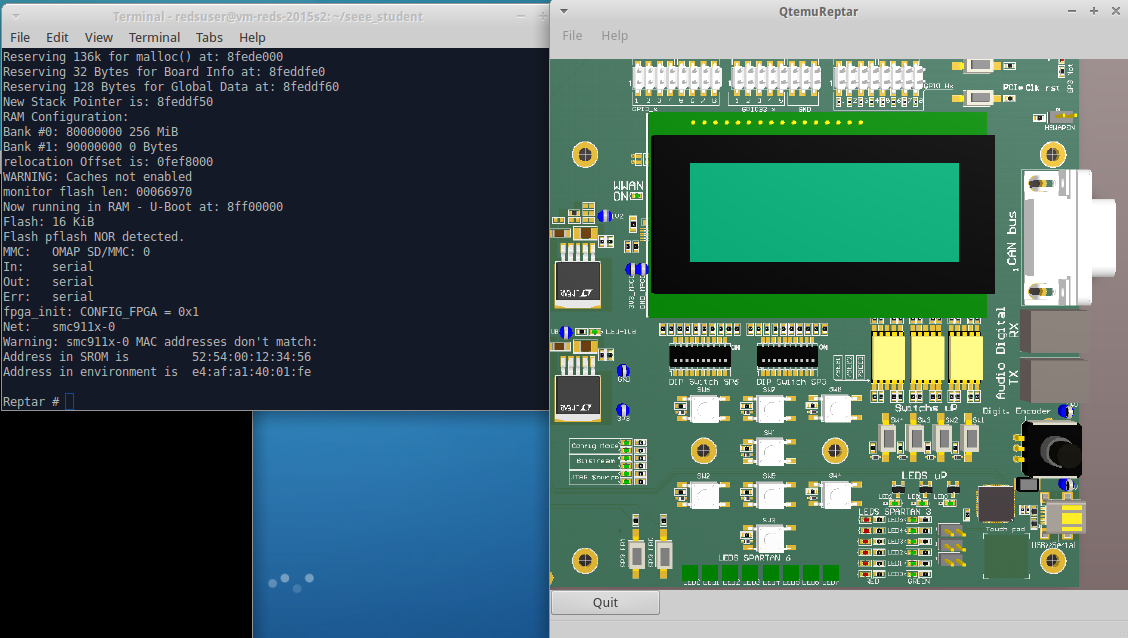
\includegraphics[width=18cm]{img/linux.png}
		\caption{Environnement émulé}
		\label{linux}
	\end{center}
\end{figure}
\textbf{e) Donnée: }Lancez votre application\\\\
\textbf{Travail réalisé: }
\begin{lstlisting}
# ls
Settings         fs               helloworld       rootfs_domU.img
# ./helloworld 
Hello world within Linux
argv[0] = ./helloworld
# 
\end{lstlisting}
\textbf{f) Donnée: }Dans Linux, tapez la commande suivante :
\begin{lstlisting}
$ /usr/share/qt/examples/effects/lighting/lighting -qws & 
\end{lstlisting}
\textbf{Travail réalisé: }Cette commande permet de lancer une application pré installée de l'émulateur.
\begin{figure}[H]
	\begin{center}
		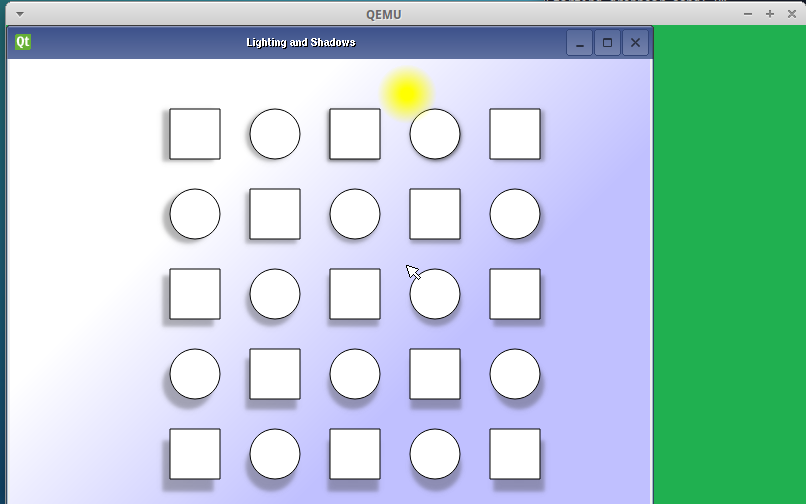
\includegraphics[width=10cm]{img/linux2.png}
		\caption{Lancement d'une application}
		\label{linux2}
	\end{center}
\end{figure}
\subsection{Tests sur la plate-forme réelle}
\textbf{a) Donnée: }Déployez l'application helloworld dans U-boot sur la plate-forme REPTAR avec l'interface réseau.
Le transfert peut s'effectuer avec la commande tftp.
Il est nécessaire d’exécuter la commande suivante pour mettre à jour les adresses IP et MAC de la plate-forme
REPTAR : 
\begin{lstlisting}
# run setmac setip 
\end{lstlisting}
\textbf{Travail réalisé: }Avec la commande tftp il faut donner comme paramètre le \textit{.bin} de l'application ainsi que l'adresse physique où charger le programme. Cette adresse est 0x81600000 comme dans les exercices précédents.
\begin{lstlisting}
redsuser@vm-reds-2015s2:~/seee_student$ cd helloworld_u-boot/
redsuser@vm-reds-2015s2:~/seee_student/helloworld_u-boot$ make
redsuser@vm-reds-2015s2:~/seee_student/helloworld_u-boot$ cp helloworld.bin /home/redsuser/tftpboot
redsuser@vm-reds-2015s2:~/seee_student/helloworld_u-boot$ sudo picocom -b 115200 /dev/ttyUSB0 
[sudo] password for redsuser: 
picocom v1.7
...
Terminal ready

Reptar # run setmac setip
Reptar # tftp 0x81600000 helloworld.bin
smc911x: detected LAN9220 controller
smc911x: phy initialized
smc911x: MAC e4:af:a1:40:01:fe
Using smc911x-0 device
TFTP from server 192.168.1.1; our IP address is 192.168.1.254
Filename 'helloworld.bin'.
Load address: 0x81600000
Loading: T #
done
Bytes transferred = 776 (308 hex)

Reptar # go 0x81600000
## Starting application at 0x81600000 ...
Example expects ABI version 6
Actual U-Boot ABI version 6
Hello World
argc = 1
argv[0] = "0x81600000"
argv[1] = "<NULL>"
Hit any key to exit ... 
\end{lstlisting}
\textbf{Remarque: }La commande tftp ne fonctionnera pas tant que la configuration réseau n'est pas correcte. Il faut impérativement que l'adresse Ip de la connexion par pont de la VM soit 192.168.1.1.
\begin{figure}[H]
	\begin{center}
		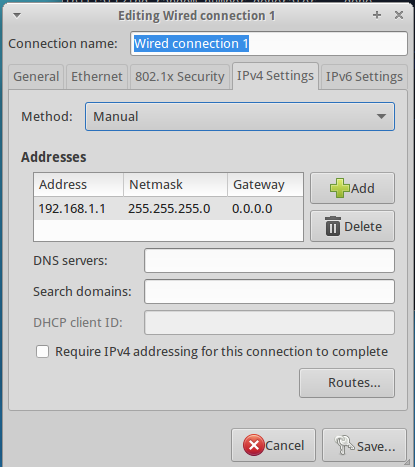
\includegraphics[width=10cm]{img/ipConfig.png}
		\caption{Configuration réseau}
		\label{ipConfig}
	\end{center}
\end{figure}
\textbf{b) Donnée: }Déployez l'application helloworld dans Linux à l'aide du réseau et de la commande scp.\\\\
\textbf{Travail réalisé: } Nous avons découvert que l'adresse Ip de la carte n'était pas celle attendue, nous avons donc dû adapter scp pour l'adresse Ip 192.168.1.254.
\begin{lstlisting}
Reptar # boot
reading uImage
...
*** Welcome on REPTAR (HEIG-VD/REDS): use root/root to log in ***
reptar login: root
Password: 
# ifconfig
eth0      Link encap:Ethernet  HWaddr E4:AF:A1:40:01:FE  
inet addr:192.168.1.254  Bcast:192.168.1.255  Mask:255.255.255.0
...
\end{lstlisting}
La commande scp permet de transférer le helloworld\_linux à la carte reptar par l'interface réseau depuis la machine hôte.
\begin{lstlisting}
redsuser@vm-reds-2015s2:~/seee_student/helloworld_linux$ scp helloworld root@192.168.1.254:helloworld

The authenticity of host '192.168.1.254 (192.168.1.254)' can't be established.
RSA key fingerprint is fb:59:a3:73:97:9d:b7:b9:8a:40:e8:bc:19:ab:ab:70.
Are you sure you want to continue connecting (yes/no)? yes
Warning: Permanently added '192.168.1.254' (RSA) to the list of known hosts.
root@192.168.1.254's password: 
helloworld                                    100% 6877     6.7KB/s   00:00    
\end{lstlisting}
L'application helloworld est maintenant chargée sur la cible, il ne reste plus qu'à l'exécuter sur celle-ci.
\begin{lstlisting}
# ls
bitstreams  helloworld     tests
# ./helloworld 
Hello world within Linux
argv[0] = ./helloworld
#
\end{lstlisting}
\subsection{Accès aux périphériques REPTAR}
\textbf{a) Donnée: } Sur la base de l’exemple gpio\_u-boot., vous devez développer une application permettant d’interagir avec les
LEDs et les switchs présents sur la carte CPU de la plate-forme REPTAR.
Le but de l’application est d’allumer une LED lorsqu’on appuie sur un switch.
\begin{enumerate}
	\item La LED 0 doit s’allumer lorsqu’on appuie sur le SWITCH 0.
	\item La LED 1 s’allume si l’on appuie sur le SWITCH 1.
	\item Et ainsi de suite pour les LEDs et switchs 0..3 de la carte CPU.
\end{enumerate}
Le switch numéro 4 sert à quitter l’application. Aidez-vous des fichiers d'en-tête (\#include) déjà présents dans
le chablon fourni.\\
L’application gpio\_u-boot est à déployer dans U-boot via la commande tftp. \\\\
\textbf{Emplacement du code réalisé: }/gpio\_u-boot.c\\\\
Ce code est très basique, mais implémente correctement les points exigés par la donnée. Les commandes suivantes ont permis de lancer l'application sur la cible réelle dans l'U-boot. Une pression sur le switch numéro 4 permet de terminer l'application.\\
\begin{lstlisting}
redsuser@vm-reds-2015s2:~/seee_student/gpio_u-boot$ make
...
redsuser@vm-reds-2015s2:~/seee_student/gpio_u-boot$ cp gpio_u-boot.bin /home/redsuser/tftpboot
redsuser@vm-reds-2015s2:~/seee_student/gpio_u-boot$ sudo picocom -b 115200 /dev/ttyUSB0 
[sudo] password for redsuser: 
picocom v1.7
...
Terminal ready

Reptar # tftp 0x81600000 gpio_u-boot.bin
smc911x: detected LAN9220 controller
smc911x: phy initialized
smc911x: MAC e4:af:a1:40:01:fe
Using smc911x-0 device
TFTP from server 192.168.1.1; our IP address is 192.168.1.254
Filename 'gpio_u-boot.bin'.
Load address: 0x81600000
Loading: T #
done
Bytes transferred = 776 (308 hex)

Reptar # go 0x81600000
...
Stop of the GPIO U-boot Standalone Application
Reptar #
\end{lstlisting}
\newpage
\section{Émulation de périphériques}
\subsection{Environnement Qemu et machine Reptar}
Cette étape vous permet de vous familiariser avec l’environnement que nous utiliserons pour
l’émulation de périphériques.
Dans cette étape, il est nécessaire de travailler avec l'application graphique Qtemu, qui constitue le
frontend graphique de Qemu. L'application est développée en C++ et utilise la librairie Qt. \\\\
\textbf{a) Donnée: }A partir du répertoire seee\_student, lancez le frontend graphique avec le script stq \\\\
\textbf{Travail réalisé: }
\begin{lstlisting}
redsuser@vm-reds-2015s2:~$ cd seee_student/
redsuser@vm-reds-2015s2:~/seee_student$ ./stq
...
Reptar # 
\end{lstlisting}
\begin{figure}[H]
	\begin{center}
		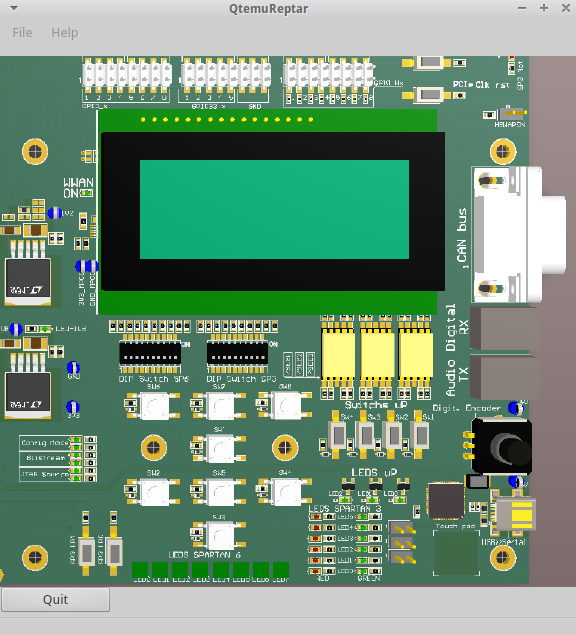
\includegraphics[width=10cm]{img/emulation1.png}
		\caption{Frontend graphique de Qemu}
		\label{emulation1}
	\end{center}
\end{figure}
\textbf{b) Donnée: }Les fichiers sources de Qemu se trouvent dans le répertoire qemu-reds. Examinez les fichiers
suivants :
\begin{enumerate}
	\item hw/arm/reptar/reptar.c Emulation plate-forme REPTAR
	\item hw/reptar\_sp6.c Emulation de la FPGA
	\item hw/reptar\_sp6\_clcd.c Emulation gestion du LCD4x20
	\item hw/reptar\_sp6\_buttons.c Emulation gestion des boutons
	\item hw/reptar\_sp6\_emul.c Gateway entre Qemu et Qtemu
\end{enumerate}
Vous trouverez également toute la documentation nécessaire sur la plate-forme Reptar dans le
répertoire doc. \\\\
\textbf{Remarque: }Ces différents fichiers implémentent ce qui ressemble à des modules noyaux.\\\\
\textbf{c) Donnée: } La compilation de Qemu pourra s'effectuer dans le répertoire qemu-reds directement, avec la
commande make (utilisez make -j4 ou -j8 pour aller plus vite !). \\\\
\textbf{Travail réalisé: }Par la suite, seule la commande \textit{make} sera nécessaire pour recompiler l'émulateur.\\
En lançant \textit{./qtemu} et Eclipse, on pourra debugger l'émulateur Qemu.
\begin{lstlisting}
redsuser@vm-reds-2015s2:~/seee_student$ cd qemu-reds/
redsuser@vm-reds-2015s2:~/seee_student/qemu-reds$ ./configure --target-list=arm-softmmu --enable-debug --disable-attr --disable-docs 
...
redsuser@vm-reds-2015s2:~/seee_student$ make -j8
...
redsuser@vm-reds-2015s2:~/seee_student$
\end{lstlisting}
\subsection{Émulation de la FPGA Spartan6}
Dans cette étape, il s'agit de mettre en place la structure nécessaire à l'émulation de la FPGA intégrée
à la plate-forme. La FPGA implémente des registres associés aux périphériques externes. Dans cette
étape, il s'agit de s'assurer que l'accès aux adresses I/O en lecture et écriture fonctionne. \\\\
\textbf{a) Donnée: }Complétez l'émulation de la FPGA afin de tester l'écriture et la lecture à l'une ou l'autre adresse
dédiée à la FPGA (affichez simplement un message). \\\\
\textbf{Emplacement du code:}\\\textit{/emulationSpartan6\_part2/reptar\_sp6.c}\\ \textit{/emulationSpartan6\_part2/reptar.c}\\\\
\textbf{Travail réalisé: }Nous avons modifié les fichiers \textit{reptar\_sp6.c} et \textit{reptar.c}\\
Le point crucial de cette partie du labo a été de trouvé l'adresse de base de la FPGA qui est \textbf{0x18000000}. Nous avons en effet besoin de cette adresse pour instancier le \textit{reptar\_sp6} dans la partie reptar. 
\begin{lstlisting}
	sysbus_create_simple("reptar_sp6",0x18000000,NULL);
\end{lstlisting}
Pour le reste de l'implémentation, nous nous somme basé sur le diagramme de séquence du support de cours et avons pris le document \textit{versatilepb.c} comme exemple pour le contenu des méthodes callback.\\
Le bon fonctionnement du code a été "testé" premièrement en réussissant la compilation sans erreurs, puis le lancement sans crash. Nous avons également ajouté des messages affichés dans la console dans les différentes méthodes callback pour suivre l'initialisation. L'exécution a été faite de la manière suivante:
\begin{lstlisting}
redsuser@vm-reds-2015s2:~$ cd seee_student/qemu-reds/
redsuser@vm-reds-2015s2:~/seee_student/qemu-reds$ make
...
redsuser@vm-reds-2015s2:~/seee_student/qemu-reds$ cd ..
redsuser@vm-reds-2015s2:~/seee_student$ ./stq
...
sp6 init
reptar-sp6-emul: sp6_emul_init
sp6 initfn
...
Reptar # 
\end{lstlisting}
\textbf{b) Donnée: }Testez les accès en lecture-écriture avec U-Boot. \\\\
\textbf{Travail réalisé: } Pour l'instant, les callback de lecture/écriture que nous avons implémentés contiennent uniquement des messages d'indication qui sont affichés dans la console. À l'aide des commandes suivantes, nous avons pu en tester le bon fonctionnement. Les commandes tentent de lire, puis écrire à l'adresse de la FPGA.
\begin{lstlisting}
Reptar # md.l 0x18000000 1
18000000:sp6 read
 00000000    ....
Reptar # mw.l 0x18000000 1
sp6 write
Reptar #
\end{lstlisting}
\subsection{Émulation des devices de type LED (output)}
\textbf{Donnée: }La FPGA est connectée à des LEDs qui sont visibles sur l'interface graphique. Cette étape consiste à
implémenter le code d'émulation précédent afin de gérer l'accès aux LEDs reliées à la FPGA.
Les interactions entre la FPGA et l'interface graphique doivent être gérées proprement. \\\\
\textbf{Emplacement du code:}\\\textit{/emulationSpartan6\_part3/reptar\_sp6.c}\\\\
\textbf{Travail réalisé: }Pour cette partie, il a fallu rechercher l'offset du registre des LEDs qui est \textit{0x003A}. Il faut donc ajouter cet offset à l'adresse de base de la FPGA. Nous avons défini une variable qui garde la valeur écrite au registre des LEDs pour permettre la relecture de la valeur. La valeur lue est simplement affichée dans la console. Nous avons ensuite implémenté la lecture et l'écriture de ce registre. Pour cela, on teste si l'offset correspond et si l'on lit/écrit des données de la bonne taille, soit 16bits. Des messages ont été implémentés pour indiquer lorsque si la lecture/écriture est faite correctement.
\\Nous avons ensuite testé le bon fonctionnement du code avec le test 10 de itbok. Le test montre que l'on arrive à lire et écrire correctement sur les leds.
\begin{figure}[H]
	\begin{center}
		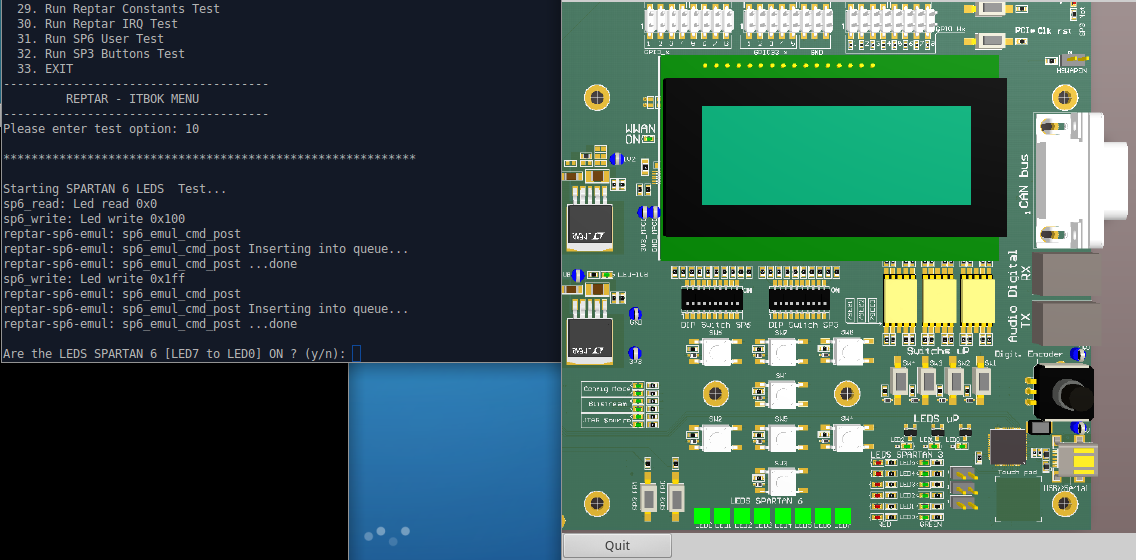
\includegraphics[width=17cm]{img/leds1.png}
		\caption{Test d'allumage des LEDs}
		\label{leds1}
	\end{center}
\end{figure}
\begin{figure}[H]
	\begin{center}
		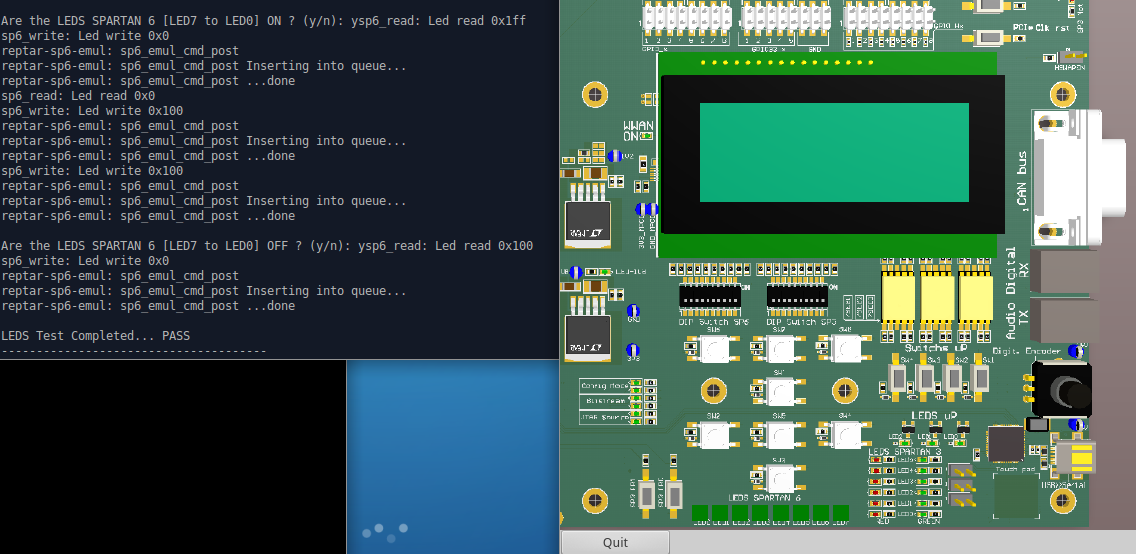
\includegraphics[width=17cm]{img/leds2.png}
		\caption{Test d'extinction des LEDs}
		\label{leds2}
	\end{center}
\end{figure}
\subsection{Émulation de type boutons (input)}
La FPGA est connectée à une série de boutons (switches) sur la plate-forme Reptar. Cette étape consiste
à mettre en place la structure nécessaire à la gestion de ces boutons. \\\\
\textbf{a) Donnée: }Adaptez les fichiers nécessaires afin que l'émulation de votre périphérique (FPGA) puisse détecter
la pression d'une touche, sans vous préoccuper pour le moment des interruptions. \\\\
\textbf{Emplacement du code:}\\\textit{/emulationSpartan6\_part4/reptar\_sp6.c}\\
\textit{/emulationSpartan6\_part4/reptar\_sp6\_buttons.c}\\\\
\textbf{Travail réalisé: }Le code de cette partie est inspiré du \textit{Guide d'utilisation de l'infrastructure}. L'offset pour lire la valeur des boutons est \textit{0x0012}. Lorsqu'un bouton est pressé, le handler du fichier sp6\_button est appelé et la valeur du registre est mémorisée. La valeur des boutons peut également être récupérée lors d'une lecture du registre \textit{0x0012}.\\\\
\textbf{b) Donnée: }Le projet sp6\_buttons\_u-boot contient une application permettant de tester vos boutons (en mode
polling). Compilez l'application et effectuez quelques tests.\\\\
\textbf{Travail réalisé: }L'application a été compilée avec make. Il faut ensuite lancer l'émulateur avec la \textit{stq}. Une fois dans l'U-boot, on peut lancer l'application testant les boutons facilement, car elle est enregistrée dans les variables d'environnements sous le nom \textit{tftp3}. Les lignes ci-dessous démontre le bon fonctionnement des boutons. Le bouton exit arrête l'application. 
\begin{lstlisting}
redsuser@vm-reds-2015s2:~/seee_student$ ./stq
...
Reptar # run tftp3
smc911x: detected LAN9118 controller
smc911x: phy initialized
smc911x: MAC e4:af:a1:40:01:fe
Using smc911x-0 device
TFTP from server 10.0.2.2; our IP address is 10.0.2.10
Filename 'sp6_buttons_u-boot/sp6_buttons.bin'.
Load address: 0x81600000
Loading: #######
done
Bytes transferred = 34512 (86d0 hex)

Reptar # run goapp
## Starting application at 0x81600000 ...
Start of the SP6 buttons standalone test application.
Button ONE pressed
...
Button ONE pressed
Button ONE pressed
Button ONE pressed
reptar-sp6-emul: sp6_emul_event_handle: read 29 
reptar-sp6-emul: sp6_emul_event_handle: cJSON_Parse done 
Button status : 0x0

Button LEFT pressed
Button LEFT pressed
Button LEFT pressed
reptar-sp6-emul: sp6_emul_event_handle: read 29 
reptar-sp6-emul: sp6_emul_event_handle: cJSON_Parse done 
Button status : 0x0

reptar-sp6-emul: sp6_emul_event_handle: read 30 
reptar-sp6-emul: sp6_emul_event_handle: cJSON_Parse done 
Button status : 0x10
Button EXIT pressed
SP6 buttons standalone test application exit.
## Application terminated, rc = 0x0
Reptar # reptar-sp6-emul: sp6_emul_event_handle: read 29 
reptar-sp6-emul: sp6_emul_event_handle: cJSON_Parse done 
Button status : 0x0
\end{lstlisting}
\subsection{Gestion des interruptions (IRQ) avec les boutons}
Complétez votre émulateur avec le code nécessaire à la gestion d'une interruption à niveau émise par
la FPGA lorsqu'un bouton est pressé. L'interruption est censée être acquittée par le driver. Il faut donc
gérer l'état interne associé à cette interruption. \\\\
\textbf{a) Donnée: }Commencez par adapter le code d'initialisation de la plate-forme (reptar.c) afin d'instancier une
interruption en provenance de la FPGA ; l'interruption sera de type niveau.\\\\
\textbf{Emplacement du code:}\\\textit{/emulationSpartan6\_part5/reptar\_sp6.c}\\
\textit{/emulationSpartan6\_part5/reptar.c}\\
\textit{/emulationSpartan6\_part5/reptar\_sp6\_buttons.c}\\\\
\textbf{Travail réalisé: }La première étape a consisté à assigner le reptar\_sp6 sur la pin GPIO 10 dans le fichier \textit{reptar.c}.\\Il a ensuite fallu faire en sorte de générer une interruption de type niveau lors d'une pression sur un bouton. Cela a été fait dans le fichier \textit{/emulationSpartan6\_part5/reptar\_sp6\_buttons.c}. Notre code génère l'interruption uniquement si les IRQ ont été préalablement autorisées en configurant les registres de contrôle. L'interruption n'est pas générée lors de la relâche du bouton (0x0), cela sert d'anti-rebond.\\
Finalement, le fichier \textit{/emulationSpartan6\_part5/reptar\_sp6.c} a été adapté pour la lecture et l'écriture du registre d'IRQ des boutons. Lorsque le registre est lu, on va lire le registre (variable) contenant l'état de bouton et l'ajouter dans le registre de status de l'IRQ, puis retourner le tout. Pour l'écriture, un masquage est fait afin de savoir si l'on veut activer et/ou quittancer les interruptions et dans ce cas repasser la GPIO10 à l'état bas.\\\\
\textbf{b) Donnée: }Testez que l'interruption fonctionne en configurant le contrôleur GPIO et en interrogeant le registre
d'état, dans U-Boot. Les registres du microcontrôleur à utiliser sont les suivants :
GPIO\_RISINGDETECT, GPIO\_IRQENABLE1 et GPIO\_IRQSTATUS1
De plus, l'interruption doit aussi être activée au niveau de la FPGA (cf documentation). \\\\
\textbf{Travail réalisé: }Notre code a dans un premier temps été testé à l'aide d'\textit{itbok} avec le test numéro 30. Cela a permis de valider le bon fonctionnement des interruptions avec tous les boutons. On peut voir que le message \textit{IRQ RAISE} ne s'affiche plus si l'on désactive les interruptions.
\begin{lstlisting}
	Press on SW7...
	reptar-sp6-emul: sp6_emul_event_handle: read 29 
	reptar-sp6-emul: sp6_emul_event_handle: cJSON_Parse done 
	Button status : 0x0
	reptar-sp6-emul: sp6_emul_event_handle: read 30 
	reptar-sp6-emul: sp6_emul_event_handle: cJSON_Parse done 
	Button status : 0x40
	IRQ RAISE
	sp6_read: Button irq status read 0x8d (button value 0x7)
	sp6_write: Button irq status write 0x81
	Enable IRQ
	Clear IRQ
	IRQ detected:
	- button: 7  ......... Test PASSED
	Press on SW8...
	reptar-sp6-emul: sp6_emul_event_handle: read 29 
	reptar-sp6-emul: sp6_emul_event_handle: cJSON_Parse done 
	Button status : 0x0
	reptar-sp6-emul: sp6_emul_event_handle: read 31 
	reptar-sp6-emul: sp6_emul_event_handle: cJSON_Parse done 
	Button status : 0x80
	IRQ RAISE
	sp6_read: Button irq status read 0x8f (button value 0x8)
	sp6_write: Button irq status write 0x81
	Enable IRQ
	Clear IRQ
	IRQ detected:
	- button: 8  ......... Test PASSED
	sp6_write: Button irq status write 0x1
	Disable IRQ
	Clear IRQ
	
	IRQ test complete. Press Enter to exit
	reptar-sp6-emul: sp6_emul_event_handle: read 29 
	reptar-sp6-emul: sp6_emul_event_handle: cJSON_Parse done 
	Button status : 0x0
	reptar-sp6-emul: sp6_emul_event_handle: read 31 
	reptar-sp6-emul: sp6_emul_event_handle: cJSON_Parse done 
	Button status : 0x80
	reptar-sp6-emul: sp6_emul_event_handle: read 29 
	reptar-sp6-emul: sp6_emul_event_handle: cJSON_Parse done 
	Button status : 0x0
\end{lstlisting}
\subsection{Émulation de l'afficheur 7 segments}
La FPGA est connectée à un afficheur 7 segments, visible sur l’émulateur. Cette étape consiste à mettre
en place la gestion de cet afficheur 7 segments.\\\\
\textbf{a) Donnée: }Adaptez les fichiers nécessaires afin que l'émulation de votre périphérique (FPGA) puisse gérer les
trois digits de l’afficheur 7 segments. \\\\
\textbf{Emplacement du code:}\textit{/emulationSpartan6\_part6/reptar\_sp6.c}\\\\
\textbf{Travail réalisé: }Pour cette partie, nous avons simplement ajouté le code pour écrire et lire dans le registre de chacun des trois digits de l'affichage 7 segments. La valeur de chaque affichage est stocké dans une variable. Pour l'écriture, il faut spécifier dans le gson le nom du périphérique, le numéro du digit ainsi que la valeur à afficher.\\\\
\textbf{b) Donnée: }Le dossier 7seg\_u-boot contient une application permettant de tester l’afficheur 7 segments : les
chiffres de 0 à 9 doivent défiler progressivement : 012, puis 123, 234, 456, 567, …, 901, 012, etc.
Compilez l'application et effectuez quelques tests.\\\\
\textbf{Travail réalisé: }Une fois l'application compilée, il a fallu la lancer dans l'U-boot. Comme elle n'est pas définie dans les variables d'environnement, il faut utiliser la commande complète. Une fois lancée, l'application va incrémenter la valeur des digits. L'image ci-dessous démontre le bon fonctionnement.
\begin{lstlisting}
redsuser@vm-reds-2015s2:~/seee_student$ ./stq
...
Reptar # tftp 7seg_u-boot/7seg_u-boot.bin
smc911x: detected LAN9118 controller
smc911x: phy initialized
smc911x: MAC e4:af:a1:40:01:fe
Using smc911x-0 device
TFTP from server 10.0.2.2; our IP address is 10.0.2.10
Filename '7seg_u-boot/7seg_u-boot.bin'.
Load address: 0x81600000
Loading: #######
done
Bytes transferred = 34932 (8874 hex)
Reptar # run goapp
\end{lstlisting}
\begin{figure}[H]
	\begin{center}
		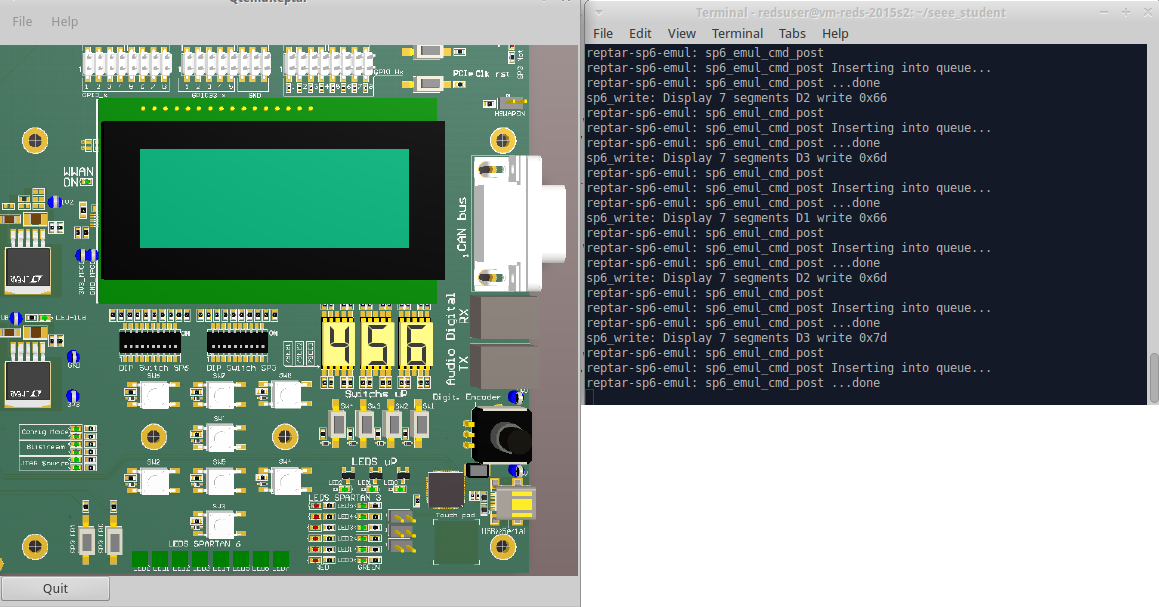
\includegraphics[width=15cm]{img/emulation2.png}
		\caption{Frontend graphique de Qemu avec affichage 7 segments}
		\label{emulation2}
	\end{center}
\end{figure}
\subsection{Mini-application utilisant les boutons et l'afficheur 7 segments}
\textbf{a) Donnée: }Le dossier miniapp\_u-boot contient un chablon. Complétez-le afin de créer une application qui
utilise les boutons SW2, SW5, SW4 et SW3, ainsi que l’afficheur 7 segments.
\begin{enumerate}
	\item Lors d’un appui sur SW2, SW5 ou SW4, le digit respectivement à gauche, au centre ou au
	milieu est incrémenté de 1, modulo 10. Si un digit atteint 9, il reviendra à 0. 
	\item La valeur initiale de chaque digit, au démarrage de l’application, est 0 (on affichera 000). 
	\item Un appui sur SW3 quitte l’application. 
	\item Vous devrez gérer l’anti-rebond : le digit ne devra être incrémenté que si le bouton est
	pressé puis relâché (comme un appui sur une touche de sonnette par exemple). \\
\end{enumerate}
\textbf{Travail réalisé: }\\\\
\textbf{b) Donnée: }Testez votre application sur l’émulateur\\\\
\textbf{Travail réalisé: }L'application a été codée avec une boucle \textit{while} exécutant de manière répétitive les étapes suivantes:
\begin{itemize}
	\item On lit le registre d'état des boutons et on stocke sa valeur dans une première variable. 
	\item On attend un petit moment.
	\item On relit le registre d'état des boutons et on stocke cette nouvelle valeur dans une seconde variable.
	\item Ensuite, on teste les deux variables avec des masques pour savoir si :
	\begin{itemize}
		\item Dans la première variable, le masquage retourne une valeur supérieure à 0 et indique que le bouton testé est enfoncé.
		\item Dans la seconde variable, le masquage retourne une valeur égale à 0 et indique que le bouton a été relâché. 
	\end{itemize}
	Ces tests sont effectués pour les trois boutons d'incrémentation des 7 segments et pour le bouton d'arrêt de l'application. 
	\item Si un des tests passe :
	\begin{itemize}
		\item Si c'est un des boutons d'incrémentation, on appelle la fonction \textit{incr\_7seg} avec en paramètre l'index du 7 segments à incrémenter.
		\item Si c'est le bouton d'arrêt, on quitte la boucle avec un \textit{break}.\\
	\end{itemize}
\end{itemize}
Nous avons remarqué une chose lors de la compilation. Il s'avère que le compilateur prend comme point d'entrée la première instruction du programme, avec le Makefile fourni. Lors des premiers essais, la fonction \textit{incr\_7seg} était implémentée avant le \textit{main}, ce qui en faisait le point d'entrée du programme. Après correction, c'est à dire, définition du prototype de la fonction avant le \textit{main} et implémentation après, tout fonctionne correctement.\\


\textbf{c) Donnée: }Déployez et testez votre application sur la plate-forme réelle\\\\
\textbf{Travail réalisé: }Une fois l'application compilée, il a fallu copier le \textit{.bin} dans le dossier \textit{tftpboot}. On peut ensuite lancer l'application depuis l'U-boot en accédant la carte Reptar avec \textit{picocom}. La pression sur le switch 3 réussit ici aussi à terminer l'application.
\begin{lstlisting}
redsuser@vm-reds-2015s2:~/seee_student$ sudo picocom -b 115200 /dev/ttyUSB0
[sudo] password for redsuser: 
...
Terminal ready

Reptar # tftp 0x81600000 miniapp_u-boot.bin
smc911x: detected LAN9220 controller
smc911x: phy initialized
smc911x: MAC e4:af:a1:40:01:0a
Using smc911x-0 device
TFTP from server 192.168.1.1; our IP address is 192.168.1.10
Filename 'miniapp_u-boot.bin'.
Load address: 0x81600000
Loading: T ###
done
Bytes transferred = 35292 (89dc hex)

Reptar # go 0x81600000
## Starting application at 0x81600000 ...
Start of the Miniapp U-boot Standalone Application
Stop of the Miniapp U-boot Standalone Application
## Application terminated, rc = 0x0
Reptar # 
\end{lstlisting}

Et ici, une photo de l'application en train de tourner sur la plateforme:
\begin{figure}[H]
    \begin{center}
        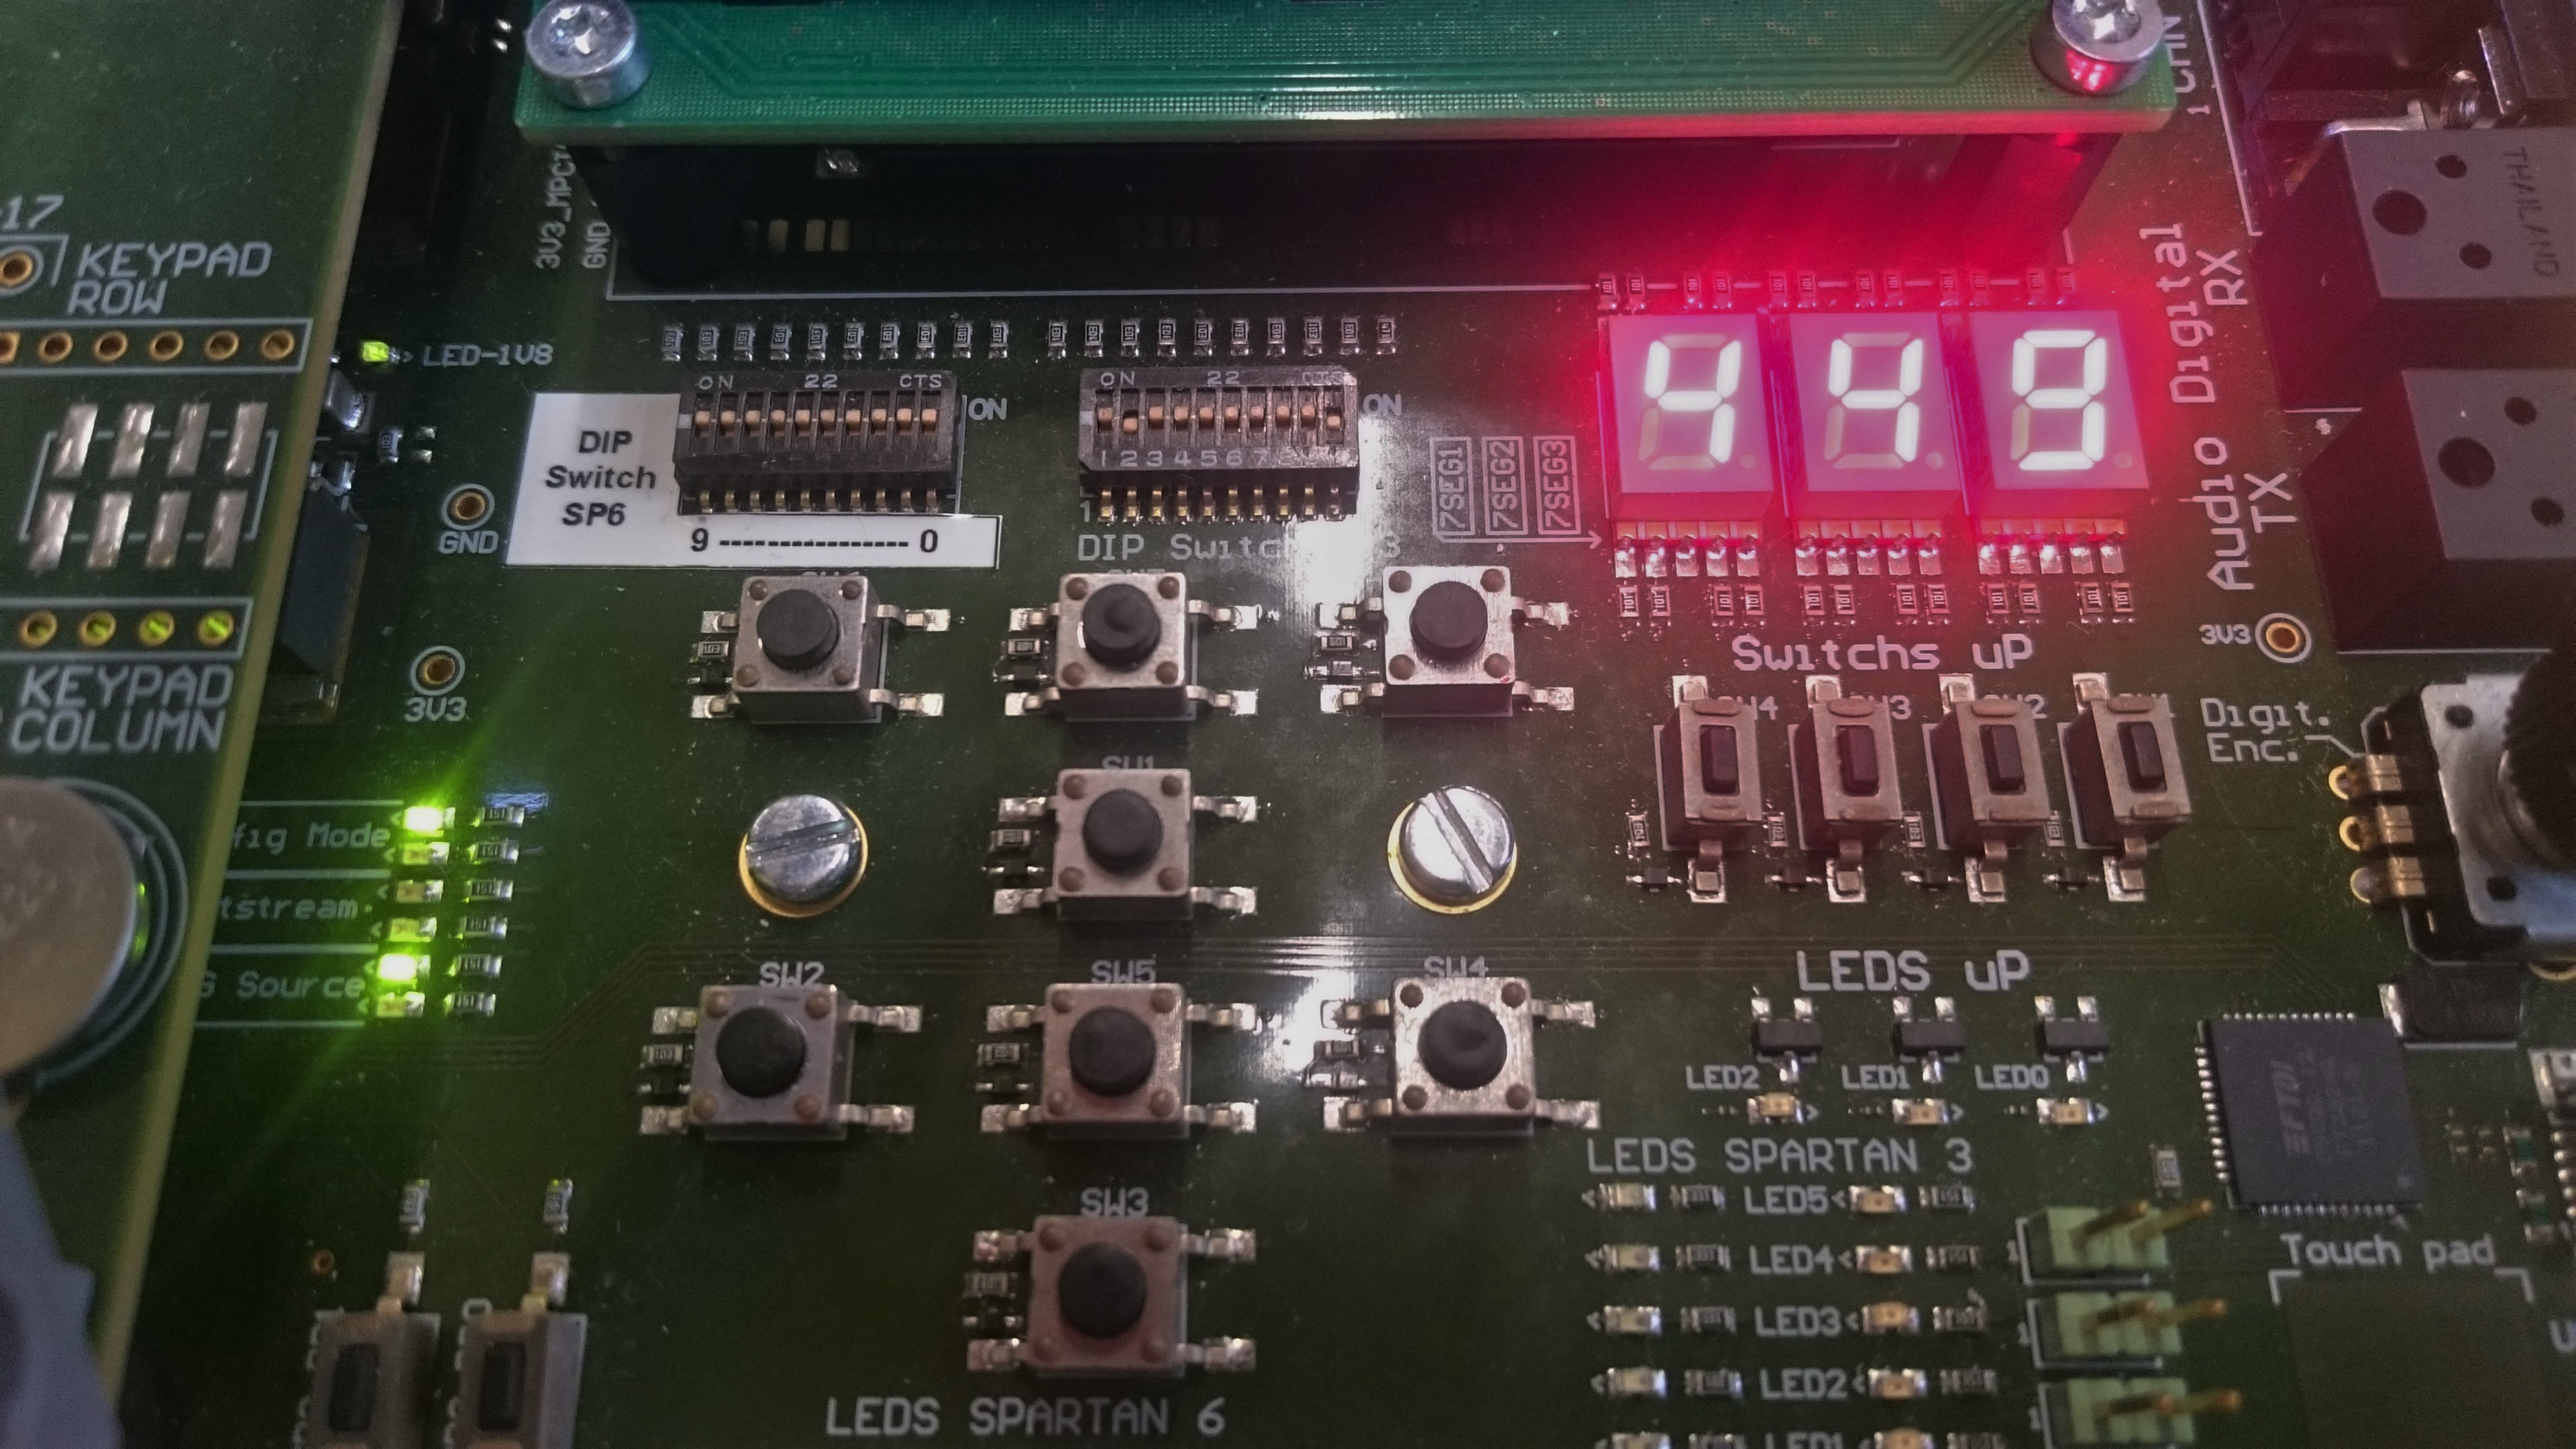
\includegraphics[width=15cm]{img/miniapp_reptar.JPG}
        \caption{Programme miniapp en fonctionnement sur la plateforme physique}
        \label{miniapp_reptar}
    \end{center}
\end{figure}

\end{document}


